%!TEX encoding = UTF-8 Unicode
%!TEX root = ./../main.tex
%!TEX TS-program = xelatex

\chapter{Inferenza Induttiva} % Main chapter title
\label{cap:uno}

Il metodo induttivo o induzione è un procedimento logico per cui dalla constatazione di fatti particolari si risale ad affermazioni o formulazioni generali.
Si suole quindi indicare con il termine induzione  il passaggio dal \textit{particolare} al \textit{generale}.
Con il termine \textbf{Inferenza Induttiva} si indica un processo che partendo da degli esempi specifici congettura delle regole generali. L'inferenza induttiva gioca un ruolo fondamentale nel più vasto scenario dell'apprendimento ed in ogni contesto che si prefigge la scoperta di strutture universali. L'applicazione di questo metodo scientifico ,intrinseco agli esseri intelligenti, all'interno delle macchine ha portato alla nascita di diversi filoni di ricerca. Uno dei più rilevanti tratta dei complessi meccanismi che consento ad un uomo di imparare un linguaggio. 

\section{Apprendimento}
 
\subsection{Definire l'apprendimento}
\label{sub:defapp}
Insieme alla capacità di pianificare cioè elaborare piani, la capacità di apprendere è ritenuta uno dei segni distintivi di un sistema intelligente. Un sistema si può considerare autonomo fintantochè le sue azioni sono determinate dalle esperienze pregresse e dalle percezioni correnti, invece che dal suo progettista (si pensi agli agenti stimolo-risposta). Senza la capacità di apprendimento un sistema non sarà in grado di operare con successo in qualsiasi ambiente ma solo in quelli previsti dal suo progettista. Nonostante la grande importanza dell'apprendimento, una conclusione largamente diffusa è che non sia possibile darne una definizione precisa: si procede invece analizzando gli effetti che l'apprendimento ha eventualmente prodotto.

Due concetti rivestono un ruolo importante nell'apprendimento: 
\begin{itemize}
\item Il miglioramento delle capacità del sistema che apprende
\item L'acquisizione di nuova conoscenza
\end{itemize}
Simon \cite{Sim83} approfondisce cosa significa migliorare le capacità di un sistema mediante l'apprendimento: \textit {L'apprendimento identifica delle modifiche in un sistema che sono adattive, nel senso che consentono al sistema di svolgere lo stesso goal, o goals analoghi, in maniera migliore nel futuro}. E' doveroso però osservare  che esistono sistemi che migliorano nel tempo senza essere soggetti a nessun processo di apprendimento e che esistono degli scenari in cui non è facile calare la definizione data da Simon.\\

L'altro fattore che contraddistingue l'apprendimento è l'acquisizione di nuove conoscenze che presuppone a monte una rappresentazione della conoscenza in maniera descrittiva o iconica per potere rappresentare la nuova conoscenza avvenuta mediante l'apprendimento.  In quest'ottica \emph{l'apprendimento è creare e modificare rappresentazioni di ciò che è stato sperimentato}. Laddove con sperimentare si intende sia l'informazione proveniente dall'apparato sensoriale dell'agente sia ciò che il sistema recepisce mediante processi interni (ad esempio ripetere più volte una frase tra sè e sè ci consente d'impararla nonostante non è avvenuto nessuno stimolo dai nostri sensi).Da questo punto di vista apprendere significa costruire una rappresentazione della realtà anzichè un miglioramento delle capacità dell'agente, aspetto quest ultimo considerato come una conseguenza.\\

E' possibile quindi constatare il grado di apprendimento di un sistema misurando i miglioramenti nel portare a compimento un certo job dopo l'apprendimento. (Miglioramenti che implicitamente sono considerati una conseguenza della rappresentazione interna dell'agente della realtà esterna). Si fa presente che in questa caratterizzazione si assume che l'agente abbia un obbiettivo e che tale obbiettivo sia conosciuto all'osservatore che valuta l'apprendimento. 
\subsection{Una possibile schematizzazione}
Esistono diverse possibilità di classificare i fattori che influenzano l’apprendimento. Michalski \cite{Mic86b} propone una divisione  basata sulle
caratteristiche del sistema che apprende.

Michalski esegue una prima distinzione in base alla quantità di conoscenze
iniziali di cui il sistema è dotato. Ai due estremi della classificazione troviamo
le reti neurali artificiali e i sistemi esperti. Nel contesto dei sistemi dotati di
scarse conoscenze iniziali le reti neurali sono uno strumento largamente usato:
le connessioni dei neuroni che costituiscono il sistema, sono determinate in
maniera essenziale dagli esempi presentati e solo marginalmente
dai valori iniziali (di solito casuali) delle connessioni. Nella progettazione di un sistema esperto invece una grande quantità di informazione viene fornita al sistema.
Un altro approccio, suggerito da Michalski, propone di suddividire i
sistemi artificiali che apprendono in base al tipo di manipolazione eseguita dal \textbf{learner}(sistema che apprende) sull’informazione proveniente dall'esterno. In ogni processo di apprendimento il \emph{learner} trasforma l’informazione fornita da un \textit{teacher}, o più in generale da un \textbf{informant} sorgente di informazione, in una nuova forma che viene poi memorizzata per usi futuri. Questa trasformazione dell’informazione, che fa uso anche delle conoscenze già possedute dal \emph{learner} viene chiamata \textbf{inferenza}. Il tipo di trasformazione eseguita determina la strategia di apprendimento di cui il sistema fa uso. Si possono distinguere,seguendo esattamente Michalski in \cite{Mic86a} , cinque diverse strategie:
\begin{itemize}
\item Apprendimento per \textit{imitazione}
\item Apprendimento per \textit{istruzioni}
\item Apprendimento per \textit{deduzione}
\item Apprendimento per \textit{analogia}
\item Apprendimento per \textit{induzione} 
\end{itemize}

Queste strategie sono elencate in ordine crescente di complessità del learning e decrescente di difficoltà del teaching.
Michalski attua questa classificazione restrigendo l'ambito di applicabilità al \textbf{\textit{concept learning}} una branca del machine learning. Un sistema intelligente deve essere abile nel classificare alcuni oggetti,eventi o comportamenti come equivalenti per raggiungere un determinato goal.  Detto in maniera succinta un sistema intelligente deve essere capace di individuare i \textit{concetti}.
\begin{definizione}
Un \textbf{concetto} è una classe di equivalenza  per cui esiste un metodo operativo che permette di discriminare le istanze come appartenenti o non appartenti al concetto.
\end{definizione} 
Dove le istanze sono le singole entità della classe di equivalenza (del concetto),cioè gli esempi  presentati dall'informant. Un \textit{learner} impara un concetto quando ,tramite una procedura effettiva, è in grado di distinguere le entità che appartengono al concetto da quelle che non appartengono.Adesso si prenderanno brevemente in esame le cinque strategie di apprendimento contestualizzandole nel \textit{concept learning}:
\begin{description}
\item[Apprendimento per imitazione] Questo è il caso estremo in cui il \textit{learner} non deve effettuare alcuna inferenza sulle informazioni che gli provengono dall' \textit{informant}. Infatti questo metodo è anche detto da Michalski impianto diretto di conoscenza (meglio conosciuto ancora come rote learning) proprio perchè il \textit{learner} non deve fare altro che inidicizzare l'informazione per poterla poi recuperare. In questo caso l'\textit{informant} fornirà una descrizione del concetto in input al \textit{learner}. Questa strategia è usata quando uno specifico algoritmo per riconoscere un concetto è implementato su un calcolatore(oppure vi è a disposizione un database di fatti che permette di riconoscere il concetto) . Ad esempio nei primi programmi che giocavano a scacchi si salvavano i risultati dell'esplorazione del grafo di  ricerca (in alcuni punti che rappresentano possibili situazioni in una partita) in un albero di gioco in modo che quando una situazione già memorizzata si fosse presentata in una partita reale si potesse risparmiare spazio e tempo di esecuzione.
\item[Apprendimento per istruzioni]In questo caso il \textit{learner} acquisisce un concetto da un \textit{teacher}, o da un’altra forma organizzata di informazione, come una publicazione o un libro, ma non copia direttamente in memoria l’informazione acquisita. Nell’apprendimento per istruzioni le trasformazioni sull’informazione eseguite dal \textit{learner} sono la selezione e la riformulazione a livello sintattico. Il processo di apprendimento può consistere
nel selezionare i fatti più importanti e poi trasformarli in una forma più appropriata. Un programma che costruisce una database di fatti e
regole sulla base di una conversazione con un utente è un esempio di sistema che apprende per istruzioni.
\item[Apprendimento per deduzione]Il \textit{learner} acquisisce un concetto deducendolo dalle conoscenze fornite dall' \textit{informant} insieme a quelle che il sistema già possedeva. Inoltre, questa strategia include ogni processo nel quale la conoscenza appresa è il risultato di una trasformazione che preserva la verità delle informazioni generate dall' \textit{informant} e di ciò che viene inferito. All’interno dell' apprendimento dei concetti, l’apprendimento per deduzione tramite il processo inferenziale trasforma una definizione non adoperabile per discriminare il concetto, in una definizione operativa adatta a questo scopo. Ad esempio dal fatto che una giarra sia un oggetto stabile e trasportabile, si può dedurre che la brocca ha un fondo piatto e un manico.
\item[Apprendimento per analogia]Il \textit{learner} acquisisce un nuovo concetto modificando la definizione di un concetto simile già noto. Anzichè formulare una descrizione del concetto ex novo, il sistema adatta una descrizione esistente modificandola appropriatamente per il nuovo scopo. Ad esempio se già si conosce una regola che definisce il concetto di arancia, per imparare il concetto di mandarino si possono notificare le differenze e le similitudini tra arancia e mandarino. L’apprendimento per analogia può essere visto come un incrocio tra l’apprendimento deduttivo e quello induttivo. Attraverso l’inferenza induttiva si possono determinare le caratteristiche generali o le trasformazioni che unificano i concetti confrontati. Poi, attraverso un’inferenza deduttiva si possono derivare le proprietà caratterizzanti possedute dal concetto che deve essere appreso
\item[Apprendimento per induzione]In questa strategia  il \textit{learner} acquisisce un concetto effettuando inferenza induttiva sui fatti forniti dall' \textit{informant} o in base a delle osservazioni su tali fatti. Esistono due differenti forme di questa strategia:
\begin{enumerate}
\item \textbf{Apprendimento da esempi}\\
Al \textit{learner} partendo da degli esempi specifici (istanze del concetto) ed eventualmente dei controntroesempi induce una descrizione del concetto catturando la struttura generale . Si assume che il concetto esiste e che esiste anche un metodo effettivo per testare l'appartenenza di un'istanza ad un concetto.  Il compito del \textit{learner} è determinare una descrizione del concetto  analizzando le singole istanze del concetto. Questa strategia è utilizzata nell' \ac{IIR} 
\item \textbf{Apprendimento per osservazione e scoperta}\\
Il \textit{learner}  analizza le entità  in input e determina che qualche sottoinsieme di queste entità può essere raggruppato in un singolo concetto.Poichè , diversamente dall'apprendimento da esempi, non c'è un \textit{teacher} che conosce in anticipo i concetti questa strategia è talvota menzionata come \emph{unsupervisioned learning}. Un esempio è il \emph{clustering} cioè il partizionamento di una collezione di oggetti all'interno di gruppi o classi che avviene in maniera gerarchica; l'eredità gioca un ruolo importante: se un entità è riconosciuta appartenere ad un determinato concetto erediterà da esso e dai concetti più in alto nella gerarchia  tutte le proprietà . Ad esempio se si apprende che Freddy è un elefante, allora si può,senza vedere Freddy, dire che ha la proboscide e tutte le proprietà degli elefanti e più in generale  anche degli erbivori e dei mammiferi.
\end{enumerate}
\end{description}

\section{Induzione}
L'induzione è quel procedimento logico che permette di passare dal particolare all'universale. Questa definizione è troppo semplice e non spiega tutte le componenti in gioco nel processo induttivo. A tal fine si seguirà ancora \cite{Mic86a}. Qui le  principali componenti induttive sono più precisamente  distinte e specificate nel contesto della manipolazione simbolica:\\

\begin {description}
\item{Dati i seguenti elementi di partenza}
\begin {itemize}
\item Gli \ac{P} che comprendono fatti, generalizzazioni intermedie, specifiche osservazioni che forniscono informazioni su oggetti,fenomeni,processi eccetera. Costituiscono l'input del processo inferenziale.
\item Le \ac{BK} che contengono concetti generali o specifici del dominio, che permettono di interpretare gli enunciati premessa e le regole rilevanti per l'inferenza. Ed includono concetti precedentemente imparati, vincoli del dominio, relazioni di causalità,goals dell'inferenza,e metodi per valutare la bontà di una congettura in base al goal (criterio di preferenza)

\end{itemize}
\item{si determina alla fine dell'inferenza induttiva}
\begin{itemize}
\item Una \ac{H} che implica gli enunciati premessa nel contesto delle conoscenze di background ed è l'ipotesi migliore in base al criterio di preferenza.
\end{itemize}
\end{description}
Si dice che \ac{H} implica fortemente  \ac{P}  nel contesto di \ac{BK} se usando \ac{BK} e l'inferenza deduttiva  \ac{P} è una conseguenza logica di \ac{H}. Schematizzando si ottiene l'equazione
\begin{equation}
\label{eqn:conslogica}
\text{\ac{H}} \,  \lor \,  \text{\ac{BK}} \implies \text{\ac{P}}
\end{equation}
che è vera con tutte le possibili \textit{interpretazioni}. In contrasto \ac{H} implica debolmente gli enunciati premessa  nel contesto delle \ac{BK} se usando le \ac{BK} e l'inferenza deduttiva \ac{P} è solo una conseguenza plausibile ma non una conseguenza logica.
Michalski fornisce un esempio di quanto appena detto:\\

\textbf{Enunciati premessa}
\begin{rientra}
 Aristotele era greco \\Socrate era greco\\Platone era greco\\
 \end{rientra}
 
\textbf{Conoscenze di background}
\begin{rientra}
Socrate, Aristotele e Platone erano filosofi \\Sono vissuti nell'antichità\\I greci sono persone\\
I filosofi sono persone\\ \emph{Criterio di preferenza}: Si preferiscono le ipotesi più corte e più utili per decidere la nazionalità dei filosofi\\
\end{rientra}

Le \textbf{ipotesi induttive} sono:
\begin{enumerate}
\item I filosofi che hanno vissuto nell'antichità erano greci
\item Tutti i filosofi sono greci
\item Tutte le persone sono greche
\end{enumerate}

L'ipotesi da preferire,in base al criterio di preferenza, è la 2, perchè è più breve della 1 e più specifica della 3; consente a differenza della 1 di determinare la nazionalità di tutti i filosofi. Si può di mostrare che questa ipotesi induttiva è un'ipotesi forte,poichè \ac{P} risulta essere una conseguenza logica di \ac{H} e delle \ac{BK}.

Supponiamo di aggiungere alla premessa gli enunciati  Locke era inglese e Hume era inglese e di modificare le \ac{BK} aggiungendo il fatto che sia Locke che Hume erano filosofi. In questo caso una ipotesi induttiva forte potrebbe essere che tutti i filosofi erano greci, con l’eccezione di Locke e Hume. Mentre una ipotesi induttiva debole potrebbe essere che alcuni filosofi erano greci. Dal fatto che Platone era un filosofo e sulla base di questa nuova ipotesi debole non consegue che Platone era greco, consegue solo che c'è la possibilità che Platone fosse greco.

Senza pretesa di esaustività si accenna ad altri tipi di inferenza presenti nel pensiero logico con lo scopo di fare emergere le peculiarità dell'inferenza induttiva. L'inferenza sta alla base dell'apprendimento. Seguendo \cite{Mic93} l'apprendimento si può sintetizzare in $apprendimento=inferenza+memorizzazione$ (definizione leggermente diversa da quella data in \ref{sub:defapp} ) quindi una completa teoria dell'apprendimento deve includere una completa teoria dell'inferenza  \cite{Mic93}. Viene innanzitutto generalizzata l'equazione \eqref{eqn:conslogica} valida solo per l'induzione  ottenendo:
\begin{equation}
\label{eqn:fond}
\text{Q} \,  \lor \,  \text{\ac{BK}} \models \text{C}
\end{equation}
detta \textbf{equazione fondamentale} per l'inferenza.
Poi Michalsky effettua una prima suddivisione tra i metodi d'inferenza:
\begin{enumerate}
\item conclusivi
\item contingenti
\end{enumerate} 
 Nel secondo caso nell' equazione \eqref{eqn:fond} C è solo una plausibile,parziale,probabilistica conseguenza logica delle \ac{BK} e di \textit{Q}. Nell'inferenza conclusiva invece la conseguenza logica è garantita.
Le proprietà dell'inferenza induttiva  sono confrontate  con quelle dell'inferenza deduttiva ed emerge che sono duali come si vede in figura \ref{fig:dedind}
\begin{figure}[htp]
	\centering
	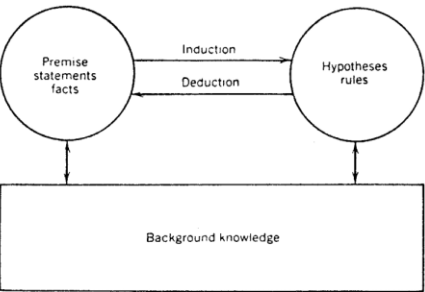
\includegraphics[ width=0.5\textwidth]{DedInd}
	\caption[Relazione tra deduzione e induzione]{Relazione tra deduzione e induzione}
   \label{fig:dedind}
\end{figure} 
La relazione logica \eqref{eqn:fond} succintamente cattura la relazione tra i due tipi d'inferenza. L'inferenza deduttiva deriva logicamente \textit{C} date \ac{BK} e \textit{Q}. L'inferenza induttiva invece va ad ipotizzare \textit{Q} date \ac{BK} e \textit{C}. La deduzione è il processo di determinare una conseguenza logica a partire da una conoscenza data, ed è \emph{truth-preserving} ( \textit{C} deve essere vero se \ac{BK} e \textit{Q} sono vere). In contrasto l'induzione sta ipotizzando un \textit{Q} che insieme con \ac{BK} implica l'input \textit{C}, ed è \emph{false-preserving} (se \textit{C} è falso  allora anche \textit{Q} deve essere falso. Cioè se  l'input in ingresso è falso anche le ipotesi congetturate saranno false). La deduzione contingente invece suona come debole in quanto è debolmente \textit{true-preserving} cioè produce conseguenze che possono essere vere in alcune situazioni e false in altre. Analogamente l'induzione contingente è debolmente \textit{false-preserving}.

In \cite{Mic93} l'inferenza viene considerata come un processo che prende in  Input un enunciato  e tramite le \ac{BK} già possedute (ed eventualmente la conoscenza dei criteri di preferenza per il goal che  permette di restringere tutte le possibili ipotesi tra le quali scegliere) fornisce un enunciato in Output .In quest'ottica le proprietà dell'induzione sono messe in risalto dal confronto con quelle della deduzione e dell'abduzione fornendo per ciascuno di essi degli esempi chiarificatori. 
\begin{enumerate}


\item DEDUZIONE tabella \ref{tab:ded}
 Riferendosi all'equazione fondamentale \eqref{eqn:fond} l'Input sta per \textit{Q} e l'Output sta per \textit{C}. L'Input consiste in enunciato che afferma l'appartenenza di un elemento \textit{a} ad \textit{X}. Le \ac{BK} sono costituite da un enunciato che assegna una certà proprietà \textit{q} agli elementi dell'insieme \textit{X}, e da una regola logica detta \textit{regola di specializzazione universale}. L'inferenza consiste solo nell'applicazione di tale regola che essendo una tautologia \footnote{E' un enunciato che ha sempre valore logico vero} fa si che il risultato dell'inferenza deduttiva assuma pure valore logico vero. Questo è un esempio di inferenza deduttiva conclusiva dato che l'Output è sempre una conseguenza logica dell'Input e delle \ac{BK}  
\begin{table}[htp]
\centering 
\begin{tabular}{|M{0.1\textwidth}|M{0.5\textwidth}|M{0.3\textwidth}|} 

\hline 
\textbf{Input} & $a \in X$ & $a$ è un elemento di $X$ \\
 \hline  
\multirow{2}*{\textbf{BK}}  &  $\forall x \in X,q(x)$  & Tutti gli elementi di $X$ hanno la proprietà $q$. \\[6ex] \cline{2-3} & $ \forall x \in X,q(x) \implies (a \in X \implies q(a))$ &  Se tutti gli elementi di $X$ hanno la proprietà $q$, allora ogni elemento di $x$, e quindi anche $a$, deve avere la proprietà $q$ \\
\hline 
\textbf{Output}  &  $q(a)$ & $a$ ha la proprietà $q$ \\
\hline 
 \end{tabular}
 \caption[Deduzione]{Deduzione}
\label{tab:ded}
\end{table} \\

\item INDUZIONE tabella \ref{tab:ind} Riferendosi all'equazione fondamentale \eqref{eqn:fond} l'Input è la conseguenza \textit{C} e l'Output è \textit{Q} (l'ipotesi).Si può dimostrare che l'Input è conseguenza logica dell'Output (l'ipotesi) e delle \ac{BK} quindi dato che l'equazione fondamentale \ref{eqn:fond} è rispettata l'inferenza è conclusiva (forte).  Infatti nel processo inferenziale è \emph{false-preserving}  se l'Input fosse falso (\textit{a} non ha la proprietà \textit{q}) allora l'Output avrebbe dovuto essere pure falso. Da rimarcare è che l'Output dell'inferenza induttiva (sia che sia conclusiva che contingente) non ha un valore di verità sempre vero ma può essere vero o falso (anche se l'Input e le \ac{BK} sono vere) da cui deriva il termine ipotesi per connotare l'Output.Essa si basa sull'assunzione che determinate regolarità osservate in un fenomeno continueranno a manifestarsi nella stessa forma anche in futuro e quindi generalizza ciò che vero per alcune istanze ad un insieme più grande. Invece nell'inferenza deduttiva  conclusiva  è garantito logicamente che l'Output assuma valore di verità vero se l'Input e le \ac{BK} sono pure vere perchè ciò che vero in generale resta vero in un caso specifico contemplato dalla regola generale. 

Nell'esempio riportato le conoscenze di \ac{BK} sono le stesse della deduzione. Tuttavia l'Output(l'ipotesi) è ottenuto tracciando all'indietro la \textit{regola di specializzazione universale}. Quindi l'inferenza consiste nel supporre l'implicazione presente nella regola di specializzazione valida anche nel verso opposto, perciò si dice che l'induzione è una regola d'inferenza all'indietro a la deduzione una regola d'inferenza in avanti.
\begin{table}[htp]
\centering 
\begin{tabular}{|M{0.1\textwidth}|M{0.5\textwidth}|M{0.3\textwidth}|} 

\hline 
\textbf{Input} & $q(a)$ & $a$ ha la proprietà $q$ \\
 \hline  
\multirow{2}*{\textbf{BK}}  &  $a \in X$  & $a$ è un elemento dell'insieme $X$. \\[6ex] \cline{2-3} & $ \forall x \in X,q(x) \implies (a \in X \implies q(a))$ &  Se tutti gli elementi di $X$ hanno la proprietà $q$, allora ogni elemento di $x$, e quindi anche $a$, deve avere la proprietà $q$ \\
\hline 
\textbf{Output}  &  $ \forall x \in X,q(x)$ & Tutti gli elementi di $X$ hanno la proprietà $q$ \\
\hline 
 \end{tabular}
 \caption[Induzione]{Induzione}
\label{tab:ind}
\end{table} \\

\item ABDUZIONE tabella \ref{tab:abd} In riferimento all'equazione \eqref{eqn:fond} l'Output è \textit{Q} e l'Input è \textit{C}.Si può dimostrare che l'Input è conseguenza logica dell'Output (l'ipotesi) e delle \ac{BK} quindi dato che l'equazione fondamentale \ref{eqn:fond} è rispettata l'inferenza è conclusiva (forte).Come nel caso dell'induzione l'inferenza abduttiva conclusiva è \textit{false-preserving}. Come nell'induzione l'Output è solo un ipotesi e quindi il suo valore di verità è incerto e c'è solo una probabilità che sia vero. L'abduzione, come l'induzione, non contiene in sé la sua validità logica e deve essere confermata per via empirica.
Nell'abduzione come nell'induzione la regola implicativa di specializzazione universale viene tracciata all'indietro. Tuttavia c'è un'importante differenza infatti nell'induzione  la regola implicativa nelle \ac{BK} costituisce una tautologia mentre nel caso dell'abduzione rappresenta una verità solo nel dominio di conoscenza e non una verità universale.

Nell'esempio specifico si assume che un elemento \textit{a} gode della proprietà \textit{q}. Le \ac{BK} consistono in un unico enunciato, che esprime il fatto che tutti gli elementi di un certo insieme \textit{X} hanno la proprietà \textit{q}. L'inferenza abduttiva produce in Output un enunciato che asserisce l'appartenenza di  \textit{a} ad  \textit{X}. Intuitivamente tutti gli elementi che appartengono ad un insieme \textit{X} hanno una proprietà; dall'input si ha che un elemento \textit{a} ha quella proprietà; siccome tutti gli elementi appartenenti all'insieme \textit{X} possiedono quella stessa proprietà si suppone che  \textit{a} appartiene all'insieme \textit{X} 
\begin{table}[htp]
\centering 
\begin{tabular}{|M{0.1\textwidth}|M{0.5\textwidth}|M{0.3\textwidth}|} 

\hline 
\textbf{Input} & $q(a)$ & $a$ ha la proprietà $q$ \\
 \hline  
\textbf{BK}  &  $\forall x,x \in X \implies q(x)$  & Se $x$ è un elemento di $X$ allora $x$ ha la proprietà $q$. \\ \cline{2-3}
\hline 
\textbf{Output}  &  $a \in X$ & $a$ è un elemento di $X$ \\
\hline 
 \end{tabular}
 \caption[Abduzione]{Abduzione}
\label{tab:abd}
\end{table} \\
\end{enumerate} 

\subsection{Metodologia di ricerca induttiva}
Si introduce brevemente,seguendo ancora \cite{Mic86a} il \textit{learning da esempi} induttivo di un concetto come un problema di ricerca in uno spazio. L'algoritmo inferenziale induttivo riceve in ingresso degli esempi (ed eventualmente anche controesempi) di membri del concetto target(specifiche istanze) sottoinsieme dello \textbf{spazio delle istanze} che costituisce l'insieme di tutte le possibili istanze osservabili. Lo \textbf{spazio dei concetti} costituisce invece l'insieme di tutti i possibili concetti (tutte le possibili soluzioni). I concetti quasi sempre necessitano di una descrizione, un linguaggio che formalmente consente di definire operativamente un concetto e per questo si parla in maniera interscambiabile di \textbf{spazio delle descrizioni}. Un concetto è consistente se accetta alcuni esempi positivi e rifiuta tutti quelli negativi; è completo invece quando accetta tutti gli esempi positivi. La macchina inferenziale induttiva ha lo scopo di selezionare un'ipotesi dallo \textbf{spazio delle ipotesi} che sia consistente e completa con gli esempi visti. Lo spazio delle ipotesi è un sottoinsieme dello spazio dei concetti. All'aumentare degli esempi visti lo spazio delle ipotesi si riduce, tuttavia le ipotesi valide possono comunque essere numerose e spesso è necessario utilizzare dei criteri di preferenza per scegliere l'ipotesi corrente. E' necessario anche definire dei criteri di terminazione per sancire la ricerca conclusa.  In sintesi il \textit{concept learning induttivo} può essere descritto come una ricerca euristica nello spazio delle descrizioni della migliore ipotesi tra tutte quelle consistenti e complete rispetto agli esempi forniti.
